\documentclass[margin=1mm]{standalone}

\input{../../tikz}
\input{../../font}
\input{../../tableau_colors}

\begin{document}

\pagestyle{empty}
\pgfdeclarelayer{background}
\pgfdeclarelayer{foreground}
\pgfsetlayers{background,main,foreground}

%\xdefinecolor{darkgreen}{RGB}{175, 193, 36}
\newcounter{cntShader}
\newcounter{cntRoot}
\setcounter{cntShader}{20}
%\def\couleur{darkgreen}

\begin{tikzpicture}
    \foreach \y in {86,38,15}{
        \setcounter{cntShader}{1}
        \coordinate (a) at (0,0);
        \coordinate (b) at (0:1);
        \foreach \x in {1,...,\y}{%
            \coordinate (c) at ($ (b)!1.25cm!270:(a) $);
            \begin{pgfonlayer}{background}
                \draw[fill=lgray!\thecntShader] (a)--(b)--(c)--cycle;
                \draw[fill=white] (a)--(b)--(c)--cycle;
            \end{pgfonlayer}
            \setcounter{cntRoot}{\x}
            \addtocounter{cntRoot}{1}
            \node[] at (c) {\includegraphics[trim={1pt 1pt 1pt 1pt},clip,width=1cm]{assembly_\thecntRoot.png}};
            \node[circ, fill opacity=0.0, fill=white, text width=0.85cm] at (c) {};
            %\node[fill=white,draw,circle,inner sep=0pt,opacity=0.1] at (c) {};
            \coordinate (b) at (c);
            \pgfmathsetcounter{cntShader}{\thecntShader+4}
            \setcounter{cntShader}{\thecntShader}
       }
    }
    \node[] at (0:1) {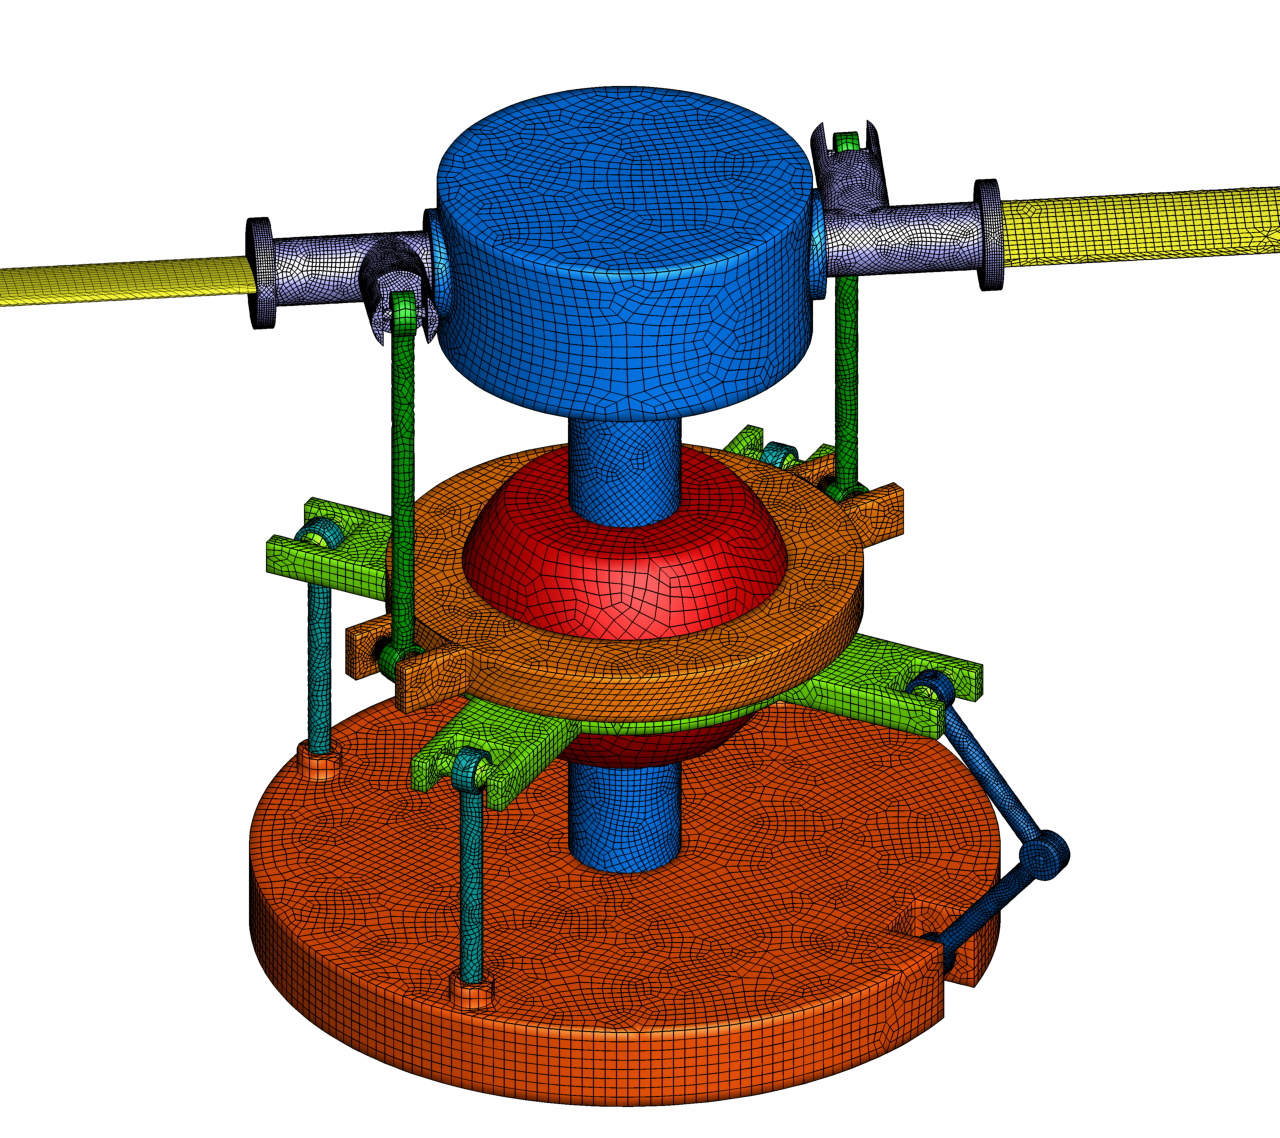
\includegraphics[trim={1pt 1pt 1pt 1pt},clip,width=1cm]{assembly_0.png}};
    \node[circ, fill opacity=0.0, fill=white, text width=0.85cm] at (0:1) {};
    %\node[fill=white,draw,circle,inner sep=0pt,opacity=0.1] at (0:1) {};
\end{tikzpicture}

\end{document} 
